\documentclass[a4paper,10pt]{article}

\usepackage{lipsum}
\usepackage[english]{babel}
\usepackage[margin=15mm]{geometry}
\usepackage{amsmath}
\usepackage{amssymb}
\usepackage{graphicx}
\usepackage{subfigure}
\usepackage{wrapfig}

\title{Multi-Agent Systems Summative Assignment}
\date{\today}
\author{James King}

\begin{document}
\maketitle

\section{Application Specification}
\subsection{Overview}
\paragraph{World.}
The task is a simple turn-based game within a tile based world, where two or more teams of bots compete for survival. Each team starts with one or more \textbf{home} tiles, upon which a bot belonging to that team begins. Every remaining tile in the world may be a solid \textbf{wall}, a \textbf{resource} item, a \textbf{bot}, or \textbf{empty}. The world is a two dimensional grid of fixed dimensions, and has the topology of the surface of a torus (travelling off one side of the grid will bring you to the opposite side). The world is initially unknown to players of the game, but at the start of each turn every player is given the state of previously undiscovered tiles that are within a certain fixed \textbf{vision radius} of any agent on their team. The locations of resources, along with the positions, team affiliation and direction of agents within the vision radius is also given before each turn.

\begin{figure}[ht]
  \centering
  \mbox{
    \subfigure
      [The blue bot moves to eliminate the pink bot.]
      {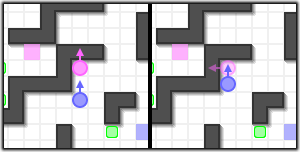
\includegraphics[width=0.45\linewidth]{kill}}
    \quad
    \subfigure
      [Mutual elimination when two bots occupy the same tile.]
      {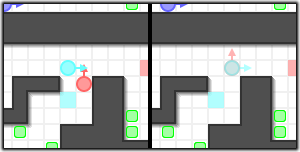
\includegraphics[width=0.45\linewidth]{mutual}}
  }
  \caption{Demonstrations of the two rules for bot elimination.}
  \vspace{-5mm}
\end{figure}

\paragraph{Bots.}
Bots have a \textbf{direction} property, which may be any one of the cardinal directions (\textbf{north}, \textbf{east}, \textbf{south}, or \textbf{west}). Each turn, each team decides a single action to perform with each bot belonging to them. This action may be to rotate the bot \textbf{left} or \textbf{right} (so a bot that was facing east which turns left will now face north), to \textbf{move} one tile in the direction it is currently facing (unless a wall is in the destination tile, in which case it does not move), or to \textbf{pass} and do nothing. After each team decides on a set of moves, all the bots commit to their assigned instruction simultaneously. If any two or more bots occupy the same tile they are removed from the world before the next turn. Also, a bot is removed if it is neighbouring another bot of a different team that is facing it.


\paragraph{Resources.}
Resources are items that appear at regular intervals in the world on randomly selected empty tiles. These are initially stationary, but if a bot appears on a neighbouring tile and faces the resource, the bot begins to \textbf{carry} the resource which will attempt to remain one tile in front of the carrying bot. If the carrying bot moves forward, the resource is \textbf{pushed} in the direction the bot moved by one tile. If the bot turns, the resource will move to whichever tile the bot is now facing. However, if the destination tile for the resource when either pushed or turned isn't vacant, the resource is removed from the world. Finally, if the resource is moved to a home tile, a new bot belonging to the home tile's corresponding team is created in its place.

\begin{figure}[ht]
  \centering
  \mbox{
    \subfigure
      [Moving a resource (green) onto a home tile spawns a new bot and consumes the resource.]
      {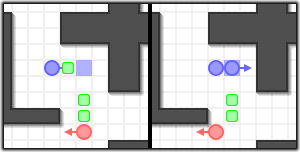
\includegraphics[width=0.45\linewidth]{capture}}
    \quad
    \subfigure
      [Pushing a resource into a wall, bot, or another resource will remove it.]
      {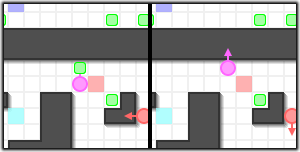
\includegraphics[width=0.45\linewidth]{destroy}}
  }
  \caption{Demonstrations of resource consumption and destruction.}
  \vspace{-5mm}
\end{figure}

\paragraph{Solution Requirements and Interfaces.}
Each team will have a single program that controls all of the bots on their team. Each program is initially given the dimensions of the world, number of teams, vision radius and allowed time per turn over standard input, and then at the start of each turn they provided with given the tile, resource and bot information as previously specified. Each team's program is then expected to produce an action for each bot over standard output, and upon the arrival of all instructions the game moves to the next turn. If any team's program fails to produce its set of actions before the allotted time has elapsed, all bots belonging to that team are eliminated and its program terminated. Each controller program may be implemented in any language that supports standard input and output operations.

\paragraph{End Conditions and Goals.}
The game lasts until either a predetermined turn limit is reached, or only bots belonging to one team remain. When the game ends, whichever team has the most remaining bots is declared the winner. The aim of the game is therefore to try and eliminate as many bots belonging to opposing teams as possible, while attempting to transport resources back to a home tile owned by your team and preventing other teams from doing so.

\subsection{Task Environment Identification}
A useful initial step when designing any kind of system involving agents is to classify the environment in terms of how it is perceived by and reacts to agents, and to recognise exactly which behaviours should be encouraged in agents. These properties of the task are usually known as the \textbf{performance measure}, \textbf{environment properties}, \textbf{actuators} and \textbf{sensors}, or the \textbf{PEAS}, as discussed by Norvig and Russel in Artificial Intelligence: A Modern Approach\cite{norvig10}.

\paragraph{Performance Measure.}
As this is a cooperative system (at least with respect to the bots belonging to one team), where the cooperating bots reside in the same program, performance may be measured for the team as a whole and not for each bot independently. Each team is attempting to maximise their number of active bots, while reducing the number of bots in opposing teams. This can be expressed as a ratio of active bots belonging to the measured team against the total number of active bots. However, this would suggest that a scenario where 5 bots are split between three teams $(A, B, C)$ using the distribution $(2, 2, 1)$ is equivalent to the distribution $(2, 3, 0)$ for team $A$. This should not be the case, as in the first scenario team $A$ is tied in first place with team $B$, but in the second scenario team $A$ is in second place and so should have a lower performance measure. One possible revised performance measure expression that resolves this is the following:

\begin{figure}[ht]
  \centering
  \begin{minipage}{0.8\textwidth}
    $$
      \text{performance}\left(\text{team}\right) \mapsto \frac
        {\left|\text{bots} \cap \text{team}\right|^2}
        {\sum_{t \in \text{teams}} \left|\text{bots} \cap \text{t}\right|^2}
    $$
    \caption{A performance measure expression that takes into account the number of bots belonging to opposing teams.}
  \end{minipage}
\end{figure}

\noindent
This performance measure can differentiate between distributions of agents between teams where the original expression could not, so eliminating bots from a larger (and therefore more threatening) opposing team would provide more utility than doing so from a small one. Maximizing this score will increase the probability of winning the game, and in fact as soon as the performance score for a given team reaches $1.0$ that team must win, because all opposing agents have been eliminated.

\paragraph{Environment Properties.}
Using the definitions provided by Russel and Norvig\cite{norvig10}, the environment is \textbf{partially observable} due to how only the contents of tiles near to bots are revealed to the team each bot belongs to. Naturally, it is a \textbf{multi-agent} system that is both \textbf{cooperative} (between agents belonging to the same team) and \textbf{competitive} (between agents belonging to distinct teams). The environment is slightly \textbf{stochastic} due to the random distribution of resources over time, and \textbf{uncertain} because of its stochastic nature, the presence of other agents, and because it is partially observable. Turns are \textbf{sequential} rather than episodic because each choice may affect every following one. Environment state and the intervals between percepts are \textbf{discrete} since the world is aligned to a grid and time is divided into turns, and the environment is mostly static except for the maximum turn time limit which renders it \textbf{semidynamic}. Finally, the outcomes of actions are \textbf{known} because they always produce an expected result for some localised aspect of the environment.

\paragraph{Actuators and Sensors.}
Each team can interact with the environment by selecting an action from the set of allowed actions for each of their bots. Percepts include several elements; first is a subset of previously undiscovered tiles revealing their state (either empty, a wall, or a home tile for a specified team), then the locations of visible bots along with their team and the direction they are facing, and finally the locations of visible resources.

\section{Scenarios}
A solution for this task should be able to act in the ways suggested in the following situations. Of course, two or more of the opportunities detailed here can crop up simultaneously, so the solution should evaluate which is expected to be more beneficial to pursue. Many more scenarios may emerge that do not fit into any of these templates, so the solution should account for unexpected events also. In the following scenarios, `bot' will refer to bots controlled by the solution program, and `opponents' will refer to the rest of the bots.

\newcommand{\scenario}[4]{
  \subsection{#1}
  \paragraph{Description.}
  #2

  \vspace{-3mm}
  \paragraph{Start Condition.}
  #3

  \vspace{2mm}
  \begin{center}
  \begin{tabular}{r l l l}
    ~ & \textbf{Steps} & \textbf{Functionality} & \textbf{Data} \\
    #4
  \end{tabular}
  \end{center}
}

\scenario{Capture Resource}{
  A resource is identified as being easy to capture, and is escorted to a home tile by a bot.
}{
  Resource seen near bot and risk is estimated to be below some threshold.
}{
  1. & Resource seen near bot & World Observation & Resources \\
  2. & Evaluated to be capturable without risk & Risk Evaluation & Opponents, World Tiles \\
  3. & Bot navigates to resource & Path Finding & World Tiles \\
  4. & Bot navigates back to a home tile & Path Finding & World Tiles \\
  5. & Resource is not pushed into walls / bots & World Observation & World Tiles \\
}

\scenario{Hinder Opponent Resource Capture}{
  A resource is identified as being easier for an opposing team to capture, and is removed by being pushed into a wall to hinder their efforts.
}{
  Resource seen near bot and risk is estimated to be below some threshold for some opposing team.
}{
  1. & Resource seen near bot & World Observation & Resources \\
  2. & Evaluated to be easier for an opponent to capture & Risk Evaluation & Opponents, World Tiles \\
  3. & Bot navigates to resource & Path Finding & World Tiles \\
  4. & Nearby wall tile found & World Observation & World Tiles \\
  5. & Bot pushes resource into wall & Path Finding & World Tiles \\
}

\scenario{Eliminate Opponent}{
  A vulnerable opponent is forced into an inescapable position, and is eliminated when the potential risk is deemed low enough.
}{
  A single opponent shares a locality with several bots on this team.
}{
  1. & Several bots encounter single opponent & World Observation & Opponents \\
  2. & Bots approach opponent when safe & Risk Evaluation & Opponents \\
  3. & Opponent becomes blocked & Opponent Consideration & Opponents, World Tiles \\
  4. & Bots await opportunity to safely strike & Risk Evaluation & Opponents
}

\scenario{Defend Trapped Bot}{
  A vulnerable bot is surrounded by opponents, but other bots arrive to assist.
}{
  A single bot shares a locality with several opponents, with other bots nearby to assist.
}{
  1. & Bot is blocked by opponents & Opponent Consideration & Opponents, World Tiles \\
  2. & Another bot approaches a blocking opponent & Path Finding & Opponents, World Tiles \\
  3. & Bot waits until opponent is vulnerable & Risk Evaluation & Opponents \\
  4. & Approaching bot strikes opponent & World Observation & Opponents \\
}

\newpage
\section{Agent Role Division}
\vspace{5mm}
\begin{figure}[ht]
  \centering
  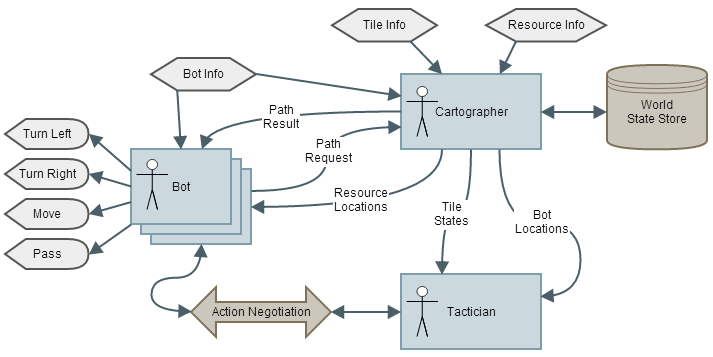
\includegraphics[width=0.8\linewidth]{interaction}
  \caption{Diagram showing the main interactions between the three proposed agent classes.}
  \vspace{-5mm}
\end{figure}
\vspace{5mm}

\paragraph{Bot Agent.}
The most obviously recognisable agent class in the system is the \textbf{Bot} agent. Each bot belonging to the team would have a separate Bot agent assigned to it, which would control self preservation of that bot and the following of any plans assigned to that bot by other agents. The Bot agent would delegate planning and most deliberation to other agents in the system, and mostly follow their instructions with some reactive mechanisms for avoiding danger. Because of this, a subsumptive architecture\cite{brooks90} would be a good fit for the overall design of the agent.

\paragraph{Cartographer Agent.}
A solution for this task should attempt to record the structure of the environment to be recalled when previously visible aspects of it are hidden. It would be wasteful for each Bot agent to hold a separate representation of the world, and so a static structure external to them would be best. While maintaining this structure is reasonably simple, an effort should be made by the solution to attempt to explore regions of the environment that were previously undiscovered, or to revisit areas to keep an eye on enemy activity. For that, a \textbf{Cartographer} agent could attempt to decide which areas are most worth visiting, and could distribute exploration tasks among Bot agents. The Cartographer would also be in charge of maintaining the world representation, and so use relevant percepts to update the structure. It would also service requests by other agents as to the state of some region of the environment. Finally, the agent could plan which resources are worth capturing or destroying, and assign agents to do either while avoiding assigning multiple agents to perform the same task. The agent would have several competing goals to achieve at any time, and should decide which to commit to. It is for this reason a Belief-Desires-Intentions\cite{rao95} architecture may be most fitting, as a subsumptive architecture is more suitable for situations where only one goal is attempted at a time.

\paragraph{Tactician Agent.}
The remaining functionality not captured by the first two agent classes relate to interaction with enemy bots, and so a \textbf{Tactician} agent may be constructed to deal with hindering, avoiding, or eliminating opposing bots. The Tactician will keep a record of the last known states of opposing bots, and also attempt to record how opponents belonging to each team react to specific situations and use that data to predict opponent actions when similar situations arise again. This agent should be able to formulate overarching plans involving many bots from the controlled team, but also respond to minor situations involving a small number of bots in a more reactive manor. A hybrid architecture with both subsumptive and BDI-oriented aspects may therefore be a useful design to use for this agent, as a purely subsumptive architecture is far too limited to account for multiple simultaneous conflict situations, but has its merits for the more reactive conflict instances.

\section{Bot Agent (Subsumptive)}

The Bot agent is the only agent that directly influences the environment. This means instances of this agent class will need to decide between acting on their own internal motives and motives of other agents that request some behaviour of them. These behaviours are described in the above diagram, and can be divided into two main behavioural groups; opponent interaction and resource retrieval / destruction.

Naturally, the opponent interaction behaviours are tied to the functions provided by the Tactician agent. These behaviours are the avoidance of elimination threats, attempted elimination of opponents, and the assistance of allied bots that are under threat. Self preservation behaviours should not be implemented as a low level layer of the subsumption stack because the Tactician may decide to commit this bot to a potentially risky move in the process of carrying out a battle manoeuvre.

\begin{figure}[!ht]
  \centering
  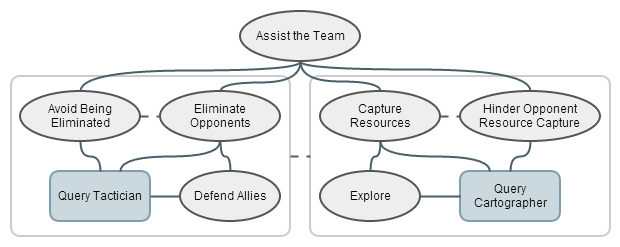
\includegraphics[width=0.8\linewidth]{bot}
  \begin{minipage}[t]{0.8\textwidth}
    \caption{A breakdown of the Bot agent's main functions into sub-functions, with possible conflicts of interest represented by dashed lines and communication with other agents as grey rectangles.}
  \end{minipage}
\end{figure}

For resource oriented functions, the Bot agent achieves its resource capture, opponent resource capture hindering, and resource discovery through exploration functionalities though goals provided by the Cartographer agent. However, the relationship between the Bot and Cartographer is a lot laxer than between the Bot and Tactician, as the Cartographer will in general only provide a general path for the Bot to follow, instead of individual actions. There may be some rare instances where the cartographer requests a specific action, so the Bot agent implementation should allow such an event.

One possible configuration of behaviour layers would be to use an \textbf{Avoid Obstacle} behaviour at the bottom of the subsumptive stack, then an \textbf{Obey Tactician Order} layer above it, followed by an \textbf{Obey Cartographer} layer, a \textbf{Follow Path} layer, and finally a \textbf{Wander} layer at the top of the stack.

\begin{wrapfigure}{r}{0.45\textwidth}
  \vspace{-5mm}
  \begin{center}
    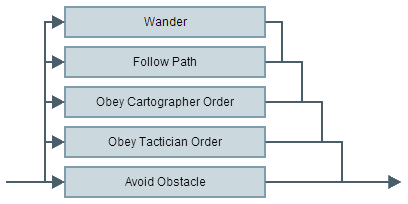
\includegraphics[width=0.43\textwidth]{subsumptive}
    \caption{Proposed layers for the Bot agent's subsumptive architecture.}
  \end{center}
  \vspace{-5mm}
\end{wrapfigure}

\paragraph{Avoid Obstacle.} This layer has highest precedence, and will respond to situations where only one action exists that could possibly be construed as rational. For example, when the bot navigates into a corner this layer will respond with an action to turn to face whichever direction isn't blocked by a wall. Implementing these kinds of reactive behaviours here will save the more computationally intensive layers from being queried. If more than one action could be interpreted as having non-negative utility this layer will abstain from making an action.

\paragraph{Obey Tactician Order.} This layer simply checks to see if the Tactician agent has assigned an order to this Bot for the current turn. If it has, that action is carried out. Otherwise the layer abstains. This layer has preference over the Obey Cartographer Layer because the survival of a bot is more critical than the exploration of the map.

\paragraph{Obey Cartographer Order.} Similarly to the Obey Tactician Order layer, this layer carries out any specific action assigned to the Bot agent by the Cartographer, if such an action has been assigned.

\paragraph{Follow Path.} The Cartographer may provide this Bot with an abstracted path to follow though the map over several turns instead of a specific action. If such a path has been provided, this layer acts to follow the path.

\paragraph{Wander.} In the event of no other layers providing an action, this layer instructs the Bot to move forwards until either an obstacle has been reached or a random variable has a value in a certain range, at which point the agent turns either left or right (preferring a direction that has no obstacle).

\section{Cartographer Agent (BDI)}
The Cartographer involves a great deal more complexity than the Bot agent, and is built around the maintenance of a knowledge base of \textbf{beliefs} that record the states of observed tiles in the world and the last known locations of resource objects. From this set of beliefs, the agent should procure a set of \textbf{desires}, beneficial future states that are evaluated to be achievable, when it decides the environment has changed sufficiently since the last desire set was generated. These desires should then be ranked, with mutually exclusive sets resolved through the dropping of some offending desires, until a set of \textbf{intentions} remain which are believed to be achievable in parallel. From these intentions \textbf{plans} are developed, which describe a method of achieving each intention through a sequence of actions performed by one or more Bot agent.

\begin{figure}[ht]
  \centering
  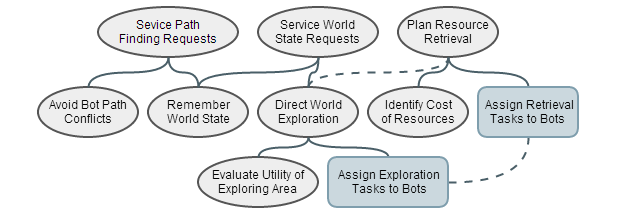
\includegraphics[width=0.8\linewidth]{cartographer}
  \begin{minipage}[t]{0.8\textwidth}
    \caption{A breakdown of the Cartographer agent's main functions into sub-functions, with possible conflicts of interest represented by dashed lines and communication with other agents as grey rectangles.}
  \end{minipage}
\end{figure}

\paragraph{Desire Generation.}
Each major element of the Cartographer's intended functionality should contribute to the pool of generated desires, assuming the environment allows for their possibility of completion. For example, each observed or remembered resource object may produce either a desire to retrieve it or a desire to destroy it (depending on the evaluated utility of either action compared to the other), and each unexplored tile of the map will produce a desire to explore it.

\paragraph{Intention Filtering.}
Intentions in this case are a filtered subset of desires without a complete formulation of a method to carry them out. The intention filtering step attempts to extract from the vast set of desires a subset that maximises utility while leaving no conflicts between any selected desires. The filtering process also respects the limited number of Bot agents that can carry out the chosen desires. In the case of several similar desires that may be achieved by one Bot simultaneously, such as exploring a group of tiles in a localised area, they may be combined into a single intention.

The exact algorithm used to decide which desires to omit and which to merge will be difficult to design optimally, but the nature of the task means that will is easy to experiment with and compare different procedures by making the alternatives compete with each other as separate teams. This should at least mean that it is possible to find some local maxima in terms of quality of filtering procedure, where only a complete redesign of the algorithm would yield better results.

\paragraph{Plan Construction.}
After the agent knows \emph{what} it wants to do, the next step is to try and work out \emph{how} to do it. At a basic level, that would require deciding which Bot agent (or agents) should be assigned a particular desire. A suitable matching between bots and desires can be found using a market clearing algorithm\cite{easley10}, where Bot agents provide valuations for each intention that are related to their expected ability to carry out that intention.

Most of the possible desires the Cartographer agent may have involve a Bot agent travelling to a position in the world of non-trivial distance from its current position. There are numerous algorithms that provide a plan for traversing the shortest path through some graph (and the tile-based grid of this environment can certainly be represented as a graph), but in particular the A* heuristic-based path finding algorithm\cite{hart68} will suffice here. The generated path does not need to specify exactly which actions a bot needs to perform to follow it, but just an abstracted route of keypoints where the path from each keypoint to the next is trivial. This allows the bot following the path to make slight diversions when avoiding obstacles, or if the bot is escorting a resource it affords the bot the freedom to avoid pushing the resource into a wall.

This stage should prove to be less troublesome to implement than the intention filtering stage, but is certainly not trivial. In particular, planning paths that take into account multiple bots moving through a confined area would require the path finding algorithm to be aware of expected future states of the environment.

\section{Tactician Agent (Hybrid)}
The final proposed agent, and possibly the most difficult to implement, is the one which handles interactions with opponent bots. This domain is rather daunting, as considering all skirmishes and sieges across the map simultaneously is a complex matter. To resolve this, for each turn \textbf{conflict instances} can be identified as separate interactions between groups of friendly and opponent bots that are independent from one another. The utility of this is plain to see, as a bot involved in a conflict on one side of the map does not need to consider enemies involved in a separate skirmish on the other.

\begin{figure}[ht]
  \centering
  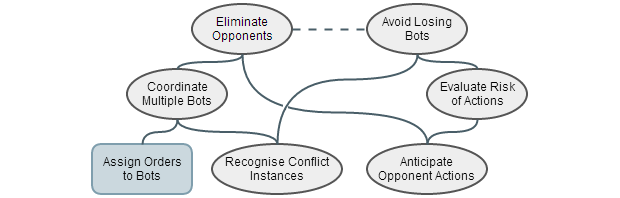
\includegraphics[width=0.8\linewidth]{tactician}
  \begin{minipage}[t]{0.8\textwidth}
    \caption{A breakdown of the Tactician agent's main functions into sub-functions, with possible conflicts of interest represented by dashed lines and communication with other agents as grey rectangles.}
  \end{minipage}
\end{figure}

After conflict instances have been distinguished, they can be tackled independently using an initially subsumptive approach. The layers with higher would be ones that recognise trivial situations resolvable in a single turn, such as avoiding a possible attack from a single opponent, or attacking an opponent in a situation with guaranteed success. However, the last layer will implement a BDI-oriented design for the recognition of and planning for more complex goals that require several turns of execution, similar to the Cartographer's structure. Delegating simpler situations to a subsumptive architecture would mean that a large number of conflict instances can be resolved without extensive processing by a BDI approach, which would assist in keeping the solution program's execution time within the enforced turn time limit.

An alternative approach to using a subsumptive / BDI hybrid design for this agent would be a Monte Carlo algorithm similar to Br\:{u}gmann's method used in his computer Go player\cite{brugmann93}. The initial step of determining separate conflict instances would be identical, but for each instance many series of randomly selected moves (for both the bots controlled by the program and opponent bots) would be emulated, with the final outcome counting towards the estimated utility of the first move in that particular sequence. The algorithm would have a fixed time limit for execution, and after that time had elapsed whichever initial set of moves has the highest estimated utility is chosen. This has a few benefits; it is far simpler to implement, guaranteed to finish execution within a given time limit, and may stumble upon an optimal set of moves that would not be apparent to a more deliberate BDI method. However, the quality of the outcome is not guaranteed in the way that the hybrid approach would at least be above some consistent minimum expected utility. This would be another case where testing the two alternatives against each other would be a useful endeavour.

\begin{thebibliography}{9}
  \bibitem{norvig10}
    S. Russell \& P. Norvig,
    \emph{Artificial Intelligence: A Modern Approach}. \newline
    Pearson Education Inc.,
    3rd Edition,
    2010.

  \bibitem{brooks90}
    R. Brooks,
    \emph{Elephants Don't Play Chess}. \newline
    Robotics and Autonomous Systems,
    Volume 6,
    1990.

  \bibitem{rao95}
    A. Rao \& M. Georgeff,
    \emph{BDI Agents: From Theory to Practice}. \newline
    Proceedings of the First International Conference on Multi-Agent Systems,
    1995.

  \bibitem{easley10}
    D. Easley \& J. Kleinberg,
    \emph{Networks, Crowds, and Markets}. \newline
    Cambridge University Press,
    2010.

  \bibitem{hart68}
    P. Hart, N. Nilsson \& B. Raphael,
    \emph{A Formal Basis for the Heuristic Determination of Minimum Cost Paths}. \newline
    IEEE Transactions on Systems Science and Cybernetics,
    Volume SSC-4,
    1968.

  \bibitem{brugmann93}
    B. Br\:{u}gmann,
    \emph{Monte Carlo Go}. \newline
    Max-Planck Institute of Physics,
    1993.
\end{thebibliography}

\end{document}
